\documentclass[aspectratio=169,xcolor=dvipsnames]{beamer}
\beamertemplatenavigationsymbolsempty
\usepackage[normalem]{ulem}
\usepackage{comp2402}
\usepackage{xmpmulti}
\renewcommand{\emph}[1]{\itshape\color{blue}#1}
\title{Interfaces/Abstract Data Types}
\author{COMP2402}
\date{}

\begin{document}

\begin{frame}
  \titlepage
\end{frame}

\begin{frame}
  \frametitle{Interfaces/Abstract Data Types}
 
  \begin{itemize}
   \item<+->Describes what a data structure \emph{does}:
     \begin{itemize}
        \item<+->supported operations (the \emph{interface})
        \item<+->meaning of operations (the \emph{semantics})
     \end{itemize}
   \item<+-> \sout{Representation and implementation}
        \end{itemize}
\end{frame}

\begin{frame}
  \frametitle{Abstract Data Types/Interfaces}

   B. Liskov and S. N. Zilles, Programming with Abstract Data Types, \emph{SIGPlan Notices}, 9(4), pp. 50-59, 1974.\\
  \begin{center}
   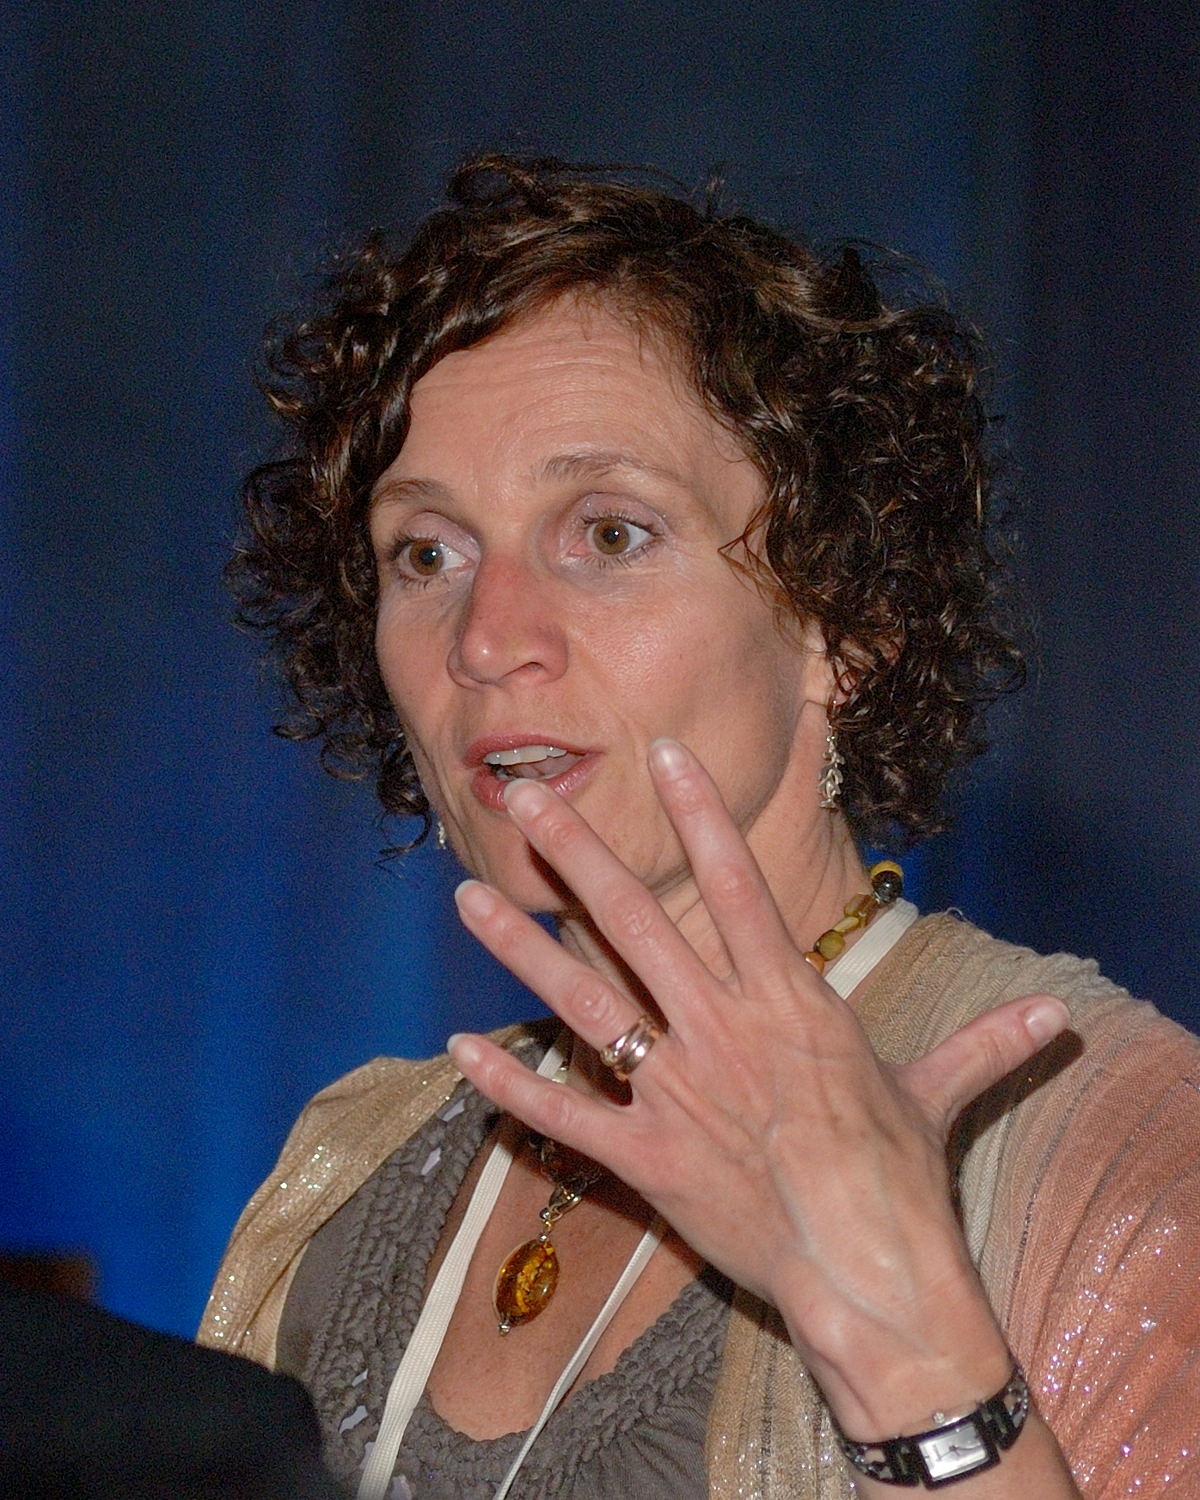
\includegraphics[height=.6\textheight]{images/liskov}\\
   B.~Liskov at the Turing Centenary Celebration (Wikimedia commons)
  \end{center}
\end{frame}

\begin{frame}
\title{The List Interface}
\maketitle
\end{frame}


\begin{frame}
  %\transdissolve[duration=0.05]
  \frametitle{The List Interface}
 
  \begin{itemize}
    \item<+-> #List#: a sequence of $n$ items\newline
    %\item<+-> Elements indexed by position, $0,\ldots,n-1$.
    \item<3-> Operations: \only<4->{#size()#}%
                        \only<5->{, #get(i)#}%
                        \only<6->{, #set(i,x)#}%
                        \only<7->{, #add(i,x)#}%
                        \only<8->{, #remove(x)#}
  \end{itemize}
     \begin{center}
      \only<1>{\includegraphics{figs/list-1}}%
      \only<2-8>{\includegraphics{figs/list-2}}%
      \only<9->{\multiinclude[<+>][format=pdf,start=5]{figs/list}}
     \end{center}

\end{frame}

\begin{frame}
  \frametitle{The USet Interface}
 
  \begin{itemize}
    \item<+-> #USet#: an \emph{unordered} collection of \emph{distinct} items\newline
    \item<3-> Operations: \only<4->{#size()#}%
                        \only<5->{, #add(x)#}%
                        \only<6->{, #remove(x)#}%
                        \only<7->{, #find(x)#}%
  \end{itemize}
     \begin{center}
      \only<1>{\includegraphics{figs/uset-1}}%
      \only<2-8>{\includegraphics{figs/uset-2}}%
      \only<9->{\multiinclude[<+>][format=pdf,start=5]{figs/list}}
     \end{center}

\end{frame}





\end{document}

